\section{Casi d'uso} 
\subsection{Attori dei casi d'uso}
\subsubsection{Attori primari}
\begin{figure}[h]
	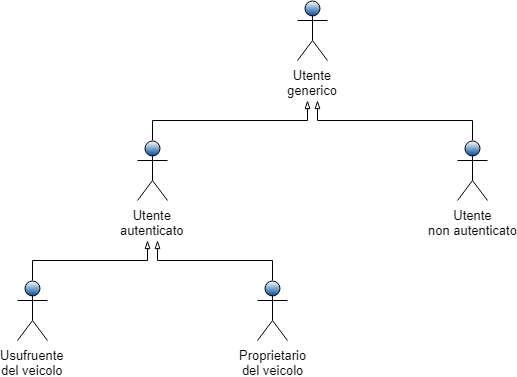
\includegraphics[width=7cm]{res/images/attori_primari.png}
	\centering
	\caption{Gerarchia degli attori primari}
\end{figure}
\begin{description}[style=nextline]
	\item[Utente generico]
	Si riferisce ad un utente generico che entra nell'applicazione.
	\item[Utente non autenticato]
	Si riferisce ad un utente generico che non ha ancora effettuato l'autenticazione nell'applicazione.
	\item[Utente autenticato]
	Si riferisce ad un utente generico che si è autenticato nell'applicazione con la procedura di login.
\end{description}

\subsection{Elenco dei casi d'uso}
In questa sezione vi sono elencati tutti i casi d'uso individuati. Ogni caso d'uso rappresenta uno scenario per uno o più attori, ovviamente applicabile anche ad eventuali attori derivati. Ogni caso d'uso, inoltre, viene descritto tramite diagrammi dei casi d'uso e possiede una precondizione seguita da una postcondizione.
\subsubsection*{Operazioni utenti}
Di seguito sono riportati tutti i casi d'uso che coinvolgono come attore primario l'utente generico, l'utente non autenticato, l'utente autenticato.
\newpage
\begin{figure}[h]
	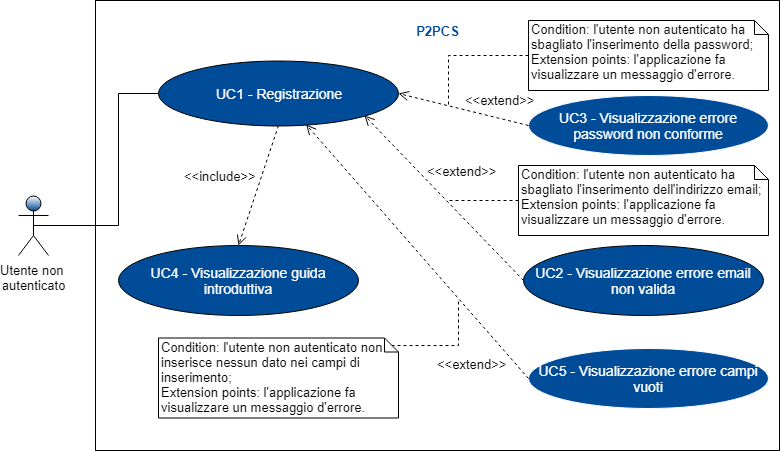
\includegraphics[width=15cm]{res/images/Schemagenerale1.png}
	\centering
	\caption{Schema generale: registrazione ed errori annessi}
\end{figure}
\subsubsection{UC1 - Registrazione}
\begin{itemize}
	\item \textbf{Attori Primari}: utente non autenticato;
	\item \textbf{Descrizione}: per effettuare il procedimento di registrazione, l'utente deve compilare tutti i campi necessari ovvero nome, cognome, email e password;
	\item \textbf{Scenario principale}: l'applicazione rende disponibili i campi da compilare per la registrazione. Dunque l'utente dovrà inserire tutti i dati necessari, quali:
		\begin{itemize}
			\item inserimento nome [UC1.1.1];
			\item inserimento cognome [UC1.1.2];
			\item inserimento indirizzo email [UC1.1.3];
			\item inserimento password [UC1.1.4];
			\item inserimento codice amico [UC1.1.5].
		\end{itemize}
	\item \textbf{Precondizione}: l'applicazione rende disponibile i campi da compilare;
	\item \textbf{Postcondizione}: l'utente viene registrato nell'applicazione;
	\item \textbf{Inclusioni}:
		\begin{itemize}
			\item visualizzazione activity introduttiva [UC4].
		\end{itemize}
	\item \textbf{Estensioni}:
		\begin{itemize}
			\item visualizzazione errore email non valida [UC2];
			\item visualizzazione errore password non conforme [UC3];
			\item visualizzazione errore campi vuoti [UC5]. 
		\end{itemize} 
\end{itemize}
\begin{figure}[h]
	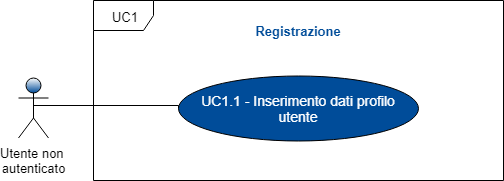
\includegraphics[width=10cm]{res/images/UC1Registrazione.png}
	\centering
	\caption{UC1 - Registrazione}
\end{figure}
\begin{figure}
	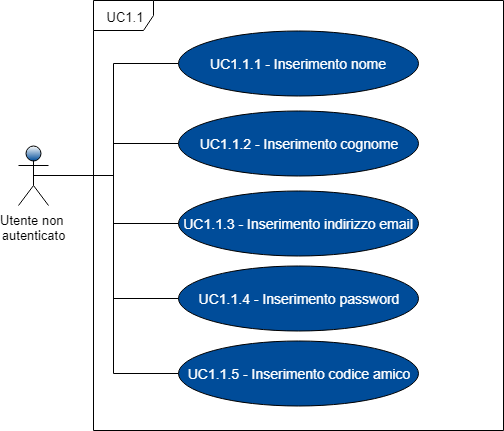
\includegraphics[width=9cm]{res/images/UC1-1Inserimento.png}
	\centering
	\caption{UC1.1 - Inserimento dati profilo utente}
\end{figure}
\subsubsection{UC1.1 - Inserimento dati profilo utente}
\begin{itemize}
	\item \textbf{Attori Primari}: utente non autenticato;
	\item \textbf{Descrizione}:l'utente compila i campi contenenti i dati relativi al profilo utente;
	\item \textbf{Scenario principale}: l'utente compila tutti i campi del form riguardanti l'account, ovvero:
		\begin{itemize}
			\item l'utente inserisce il proprio nome [UC1.1.1];
			\item l'utente inserisce il proprio cognome [UC1.1.2];
			\item l'utente inserisce l'email da associare all'account [UC1.1.3];
			\item l'utente inserisce la password da associare all'account [UC1.1.4].
		\end{itemize}
	\item \textbf{Precondizione}: l'utente è entrato nell'activity\glosp di registrazione;
	\item \textbf{Postcondizione}: l'utente ha compilato tutti i campi richiesti dalla registrazione.
\end{itemize}
\newpage
\subsubsection{UC1.1.1 - Inserimento nome}
\begin{itemize}
	\item \textbf{Attori Primari}: utente non autenticato;
	\item \textbf{Descrizione}: al fine di portare a termine il processo di registrazione l'utente deve inserire il proprio nome, campo ritenuto obbligatorio;
	\item \textbf{Scenario principale}: l'utente compila il campo relativo al nome;	
	\item \textbf{Precondizione}: l'applicazione ha reso disponibile il campo per l'inserimento del nome;
	\item \textbf{Postcondizione}: l'utente ha compilato il campo con il proprio nome.	
\end{itemize}
\subsubsection{UC1.1.2 - Inserimento cognome}
\begin{itemize}
	\item \textbf{Attori Primari}: utente non autenticato;
	\item \textbf{Descrizione}: al fine di portare a termine il processo di registrazione l'utente deve inserire il proprio cognome, campo ritenuto obbligatorio;
	\item \textbf{Scenario principale}: l'utente compila il campo relativo al cognome;	
	\item \textbf{Precondizione}: l'applicazione ha reso disponibile il campo per l'inserimento del cognome;
	\item \textbf{Postcondizione}: l'utente ha compilato il campo con il proprio cognome.	
\end{itemize}
\subsubsection{UC1.1.3 - Inserimento indirizzo email}
\begin{itemize}
	\item \textbf{Attori Primari}: utente non autenticato;
	\item \textbf{Descrizione}: al fine di portare a termine il processo di registrazione l'utente deve inserire il proprio indirizzo email, campo ritenuto obbligatorio;
	\item \textbf{Scenario principale}: l'utente compila il campo relativo all'indirizzo email;	
	\item \textbf{Precondizione}: l'applicazione ha reso disponibile il campo per l'inserimento dell'indirizzo email;
	\item \textbf{Postcondizione}: l'utente ha compilato il campo con il proprio indirizzo email.
\end{itemize}
\subsubsection{UC1.1.4 - Inserimento password}
\begin{itemize}
	\item \textbf{Attori Primari}: utente non autenticato;
	\item \textbf{Descrizione}: al fine di portare a termine il processo di registrazione l'utente deve inserire una password, campo ritenuto obbligatorio;
	\item \textbf{Scenario principale}: l'utente compila il campo relativo alla password;	
	\item \textbf{Precondizione}: l'applicazione ha reso disponibile il campo per l'inserimento della password;
	\item \textbf{Postcondizione}: l'utente ha compilato il campo con una password.
\end{itemize}

\subsubsection{UC1.1.5 - Inserimento codice amico}
\begin{itemize}
	\item \textbf{Attori Primari}: utente non autenticato;
	\item \textbf{Descrizione}: al fine di portare a termine il processo di registrazione l'utente può inserire un "codice amico", qualora ne fosse in possesso, campo ritenuto non obbligatorio;
	\item \textbf{Scenario principale}: l'utente può compilare il campo relativo al codice amico se in possesso di un codice personale inviato da un altro utente che usufruisce dell'applicazione;	
	\item \textbf{Precondizione}: l'applicazione ha reso disponibile il campo per l'inserimento del codice amico;
	\item \textbf{Postcondizione}: l'utente ha compilato il campo con un codice amico.
\end{itemize}

\subsubsection{UC1.2 - Invio dati}
\begin{itemize}
	\item \textbf{Attori Primari}: utente non autenticato;
	\item \textbf{Descrizione}: l'utente preme il pulsante per la conferma e l'invio dei dati; l'utente verrà rimandato a una nuova activity\glosp che confermerà il successo dell'operazione;
	\item \textbf{Scenario principale}: l'utente preme il pulsante di verifica ed invio dei dati;	
	\item \textbf{Precondizione}: i campi dati necessari per la registrazione sono compilabili. È presente il pulsante per la conferma dei dati;
	\item \textbf{Postcondizione}: l'utente viene rimandato a una nuova activity che conferma il successo dell'operazione e avvisa l'utente di controllare la propria e-mail per confermare il processo di registrazione.
\end{itemize}

\subsubsection{UC2 - Visualizzazione errore email non valida}
\begin{itemize}
	\item \textbf{Attori Primari}: utente non autenticato;
	\item \textbf{Descrizione}: l'utente visualizza un messaggio d'errore in quanto l'email digitata è scorretta;
	\item \textbf{Scenario principale}: l'utente non ancora autenticato tenta di registrarsi inserendo un indirizzo email non valido;
	\item \textbf{Precondizione}: l'utente non autenticato ha sbagliato l'inserimento dell'indirizzo email; 
	\item \textbf{Postcondizione}: l'applicazione fa visualizzare un messaggio d'errore.
\end{itemize}

\subsubsection{UC3 - Visualizzazione errore password non conforme}
\begin{itemize}
	\item \textbf{Attori Primari}: utente non autenticato;
	\item \textbf{Descrizione}: l'utente visualizza un messaggio d'errore in quanto la password digitata non è conforme ai seguenti vincoli:
		\begin{itemize}
			\item ci deve essere almeno una lettera maiuscola;
			\item ci deve essere almeno un carattere speciale;
			\item ci devono essere almeno 8 caratteri;
		\end{itemize}
	\item \textbf{Scenario principale}: l'utente non ancora autenticato tenta di registrarsi inserendo un password errata;
	\item \textbf{Precondizione}: l'utente non autenticato ha sbagliato l'inserimento della password; 
	\item \textbf{Postcondizione}: l'applicazione fa visualizzare un messaggio d'errore.
\end{itemize}

\subsubsection{UC4 - Visualizzazione activity introduttiva}
\begin{itemize}
	\item \textbf{Attori Primari}: utente non autenticato;
	\item \textbf{Descrizione}: l'utente visualizza una guida introduttiva che mostra le funzionalità dell'applicazione nella sue sezioni principali al termine della quale potrà accedere all'activity\glosp di login;
	\item \textbf{Scenario principale}: l'utente accede all'activity introduttiva dell'applicazione e può decidere se visualizzarla o saltarla andando ad effettuare l'accesso;
	\item \textbf{Precondizione}: l'utente si è registrato e può accedere all'activity introduttiva dell'applicazione;
	\item \textbf{Postcondizione}: il sistema fornisce all'utente la possibilità di visualizzare interamente la guida o di saltarla e raggiungere l'activity di login.
\end{itemize}

\subsubsection{UC5 - Visualizzazione errore campi vuoti}
\begin{itemize}
	\item \textbf{Attori Primari}: utente non autenticato;
	\item \textbf{Descrizione}: l'utente visualizza un messaggio d'errore in quanto non sono stati riempiti i campi di inserimento email e password;
	\item \textbf{Scenario principale}: l'utente non ancora autenticato tenta di accedere non inserendo un indirizzo email e password;	
	\item \textbf{Precondizione}: l'utente non autenticato non inserisce nessun dato nei campi di inserimento;
	\item \textbf{Postcondizione}: l'applicazione fa visualizzare un messaggio d'errore.
\end{itemize}
\begin{figure}[h]
	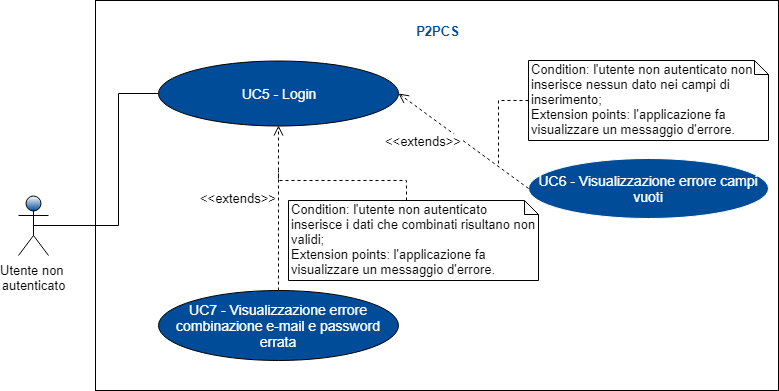
\includegraphics[width=16cm]{res/images/Schemagenerale2.png}
	\centering
	\caption{Schema generale: login ed errori annessi}
\end{figure}
\newpage
\subsubsection{UC6 - Login}
\begin{itemize}
	\item \textbf{Attori Primari}: utente non autenticato;
	\item \textbf{Descrizione}: per effettuare il procedimento di autenticazione, l'utente deve compilare i campi necessari ovvero e-mail e password;
	\item \textbf{Scenario principale}: l'applicazione rende disponibili i campi da compilare per l'autenticazione. Dunque l'utente dovrà inserire tutti i dati necessari;
	\item \textbf{Precondizione}: l'applicazione rende disponibile i campi da compilare;
	\item \textbf{Postcondizione}: dopo aver controllato che i campi sono stati compilati correttamente, l'utente viene autenticato nell'applicazione.
	\item \textbf{Estensioni}:
		\begin{itemize}
			\item visualizzazione errore campi vuoti [UC5];
			\item visualizzazione errore combinazione email e password errata [UC7];
			\item recupero password [UC8].
		\end{itemize}	
\end{itemize}
\begin{figure}[h]
	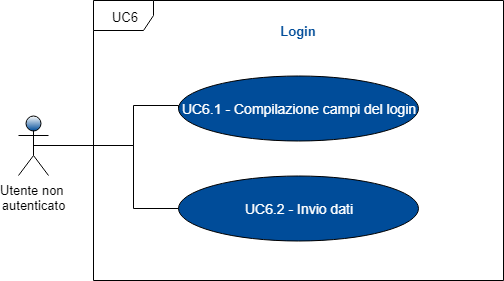
\includegraphics[width=11cm]{res/images/UC6Login.png}
	\centering
	\caption{UC6 - Login}
\end{figure}
\newpage
\subsubsection{UC6.1 - Compilazione campi per il login}
\begin{itemize}
	\item \textbf{Attori Primari}: utente non autenticato;
	\item \textbf{Descrizione}: l'utente compila i campi richiesti per l'autenticazione;
	\item \textbf{Scenario principale}: l'utente compila i campi necessari all'autenticazione ovvero:
		\begin{itemize}
			\item l'utente inserisce l'email associata al proprio account [UC5.1.1];
			\item l'utente inserisce la password associata la proprio account [UC5.1.2].
		\end{itemize}	
	\item \textbf{Precondizione}: l'utente si trova nell'activity\glosp di autenticazione;
	\item \textbf{Postcondizione}: l'utente ha compilato tutti i campi necessari all'autenticazione.	
\end{itemize}
\begin{figure}[h]
	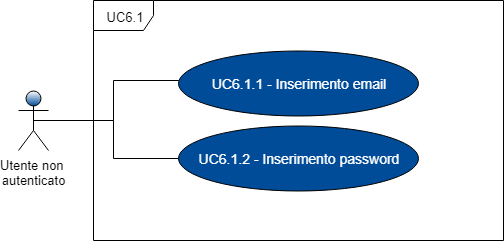
\includegraphics[width=11cm]{res/images/UC6-1Compilazione.png}
	\centering
	\caption{UC6.1 - Compilazione campi per il login}
\end{figure}
\subsubsection{UC6.1.1 - Inserimento email}
\begin{itemize}
	\item \textbf{Attori Primari}: utente non autenticato;
	\item \textbf{Descrizione}: al fine di portare a termine il processo di autenticazione l'utente deve inserire l'indirizzo email associato all'account, campo ritenuto obbligatorio;
	\item \textbf{Scenario principale}: l'utente compila il campo relativo all'indirizzo email;	
	\item \textbf{Precondizione}: l'applicazione ha reso disponibile il campo per l'inserimento dell'indirizzo email;
	\item \textbf{Postcondizione}: l'utente ha compilato il campo con l'indirizzo email associato al proprio account.
\end{itemize}

\subsubsection{UC6.1.2 - Inserimento password}
\begin{itemize}
	\item \textbf{Attori Primari}: utente non autenticato;
	\item \textbf{Descrizione}: al fine di portare a termine il processo di autenticazione l'utente deve inserire la password associata al proprio account, campo ritenuto obbligatorio;
	\item \textbf{Scenario principale}: l'utente compila il campo relativo alla password;	
	\item \textbf{Precondizione}: l'applicazione ha reso disponibile il campo per l'inserimento della password;
	\item \textbf{Postcondizione}: l'utente ha compilato il campo con la password associata al proprio account.
\end{itemize}

\subsubsection{UC6.2 - Invio dati}
\begin{itemize}
	\item \textbf{Attori Primari}: utente non autenticato;
	\item \textbf{Descrizione}: l'utente preme il pulsante per la conferma e l'invio dei dati; se email e password risulteranno corrette l'utente verrà autenticato;
	\item \textbf{Scenario principale}: l'utente preme il pulsante di verifica ed invio dei dati;	
	\item \textbf{Precondizione}: i campi dati necessari per l'autenticazione sono compilabili. È presente il pulsante per la conferma dei dati;
	\item \textbf{Postcondizione}: l'utente viene autenticato e rimandato all'activity\glosp per la gestione dei veicoli.
\end{itemize}

\subsubsection{UC7 - Visualizzazione errore combinazione email e password errata}
\begin{itemize}
	\item \textbf{Attori Primari}: utente non autenticato;
	\item \textbf{Descrizione}: l'utente visualizza un messaggio d'errore in quanto i campi di inserimento email e password sono stati riempiti in modo errato;
	\item \textbf{Scenario principale}: l'utente non ancora autenticato tenta di accedere inserendo un indirizzo email e password che insieme risultano non validi;	
	\item \textbf{Precondizione}: l'utente non autenticato inserisce i dati che combinati risultano non validi;
	\item \textbf{Postcondizione}: l'applicazione fa visualizzare un messaggio d'errore.
\end{itemize}
\newpage
\begin{figure}[h]
	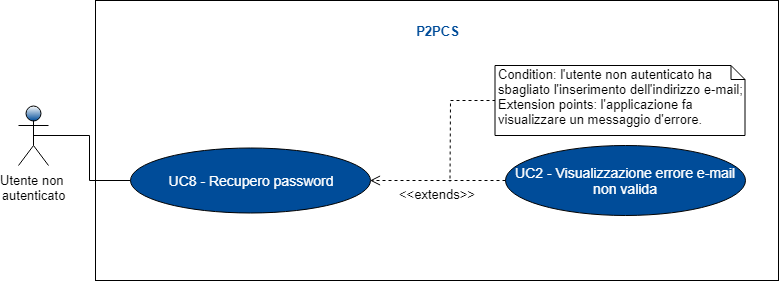
\includegraphics[width=15cm]{res/images/Schemagenerale3.png}
	\centering
	\caption{Schema generale: recupero password ed errori annessi}
\end{figure}
\subsubsection{UC8 - Recupero password}
\begin{itemize}
	\item \textbf{Attori Primari}: utente non autenticato;
	\item \textbf{Descrizione}: l'utente non autenticato non si ricorda la propria password per accedere all'account e ne richiede il recupero che avviene inserendo un'indirizzo email dove verrà inviata una nuova password;
	\item \textbf{Scenario principale}: l'utente non ancora autenticato inserisce un'indirizzo email dove potrà ricevere la nuova password da utilizzare per accedere al proprio account; 
	\item \textbf{Precondizione}: l'utente non autenticato non ricorda la password di accesso e indica un'indirizzo email di recupero;
	\item \textbf{Postcondizione}: l'utente riceve la nuova password tramite posta all'indirizzo email inviato.
	\item \textbf{Estensione}:
		\begin{itemize}
			\item visualizzazione errore email non valida [UC2].
		\end{itemize}
\end{itemize}
\begin{figure}[h]
	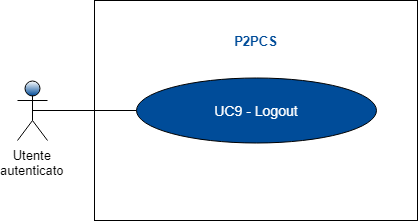
\includegraphics[width=9cm]{res/images/UC9Logout.png}
	\centering
	\caption{Schema generale: logout}
\end{figure}
\subsubsection{UC9 - Logout}
\begin{itemize}
	\item \textbf{Attori Primari}:
	utente autenticato;
	\item \textbf{Descrizione}: l'utente dal fragment\glosp Area Personale richiede il logout dall'applicazione;
	\item \textbf{Scenario principale}: l'utente è autenticato nell'applicazione e richiede di effettuare il logout, premendo sull'apposito pulsante;
	\item \textbf{Precondizione}: l'utente ha effettuato il login all'applicazione e richiede di essere disconnesso dall'applicazione;
	\item \textbf{Postcondizione}: l'utente viene disautenticato e rimandato all'activity\glosp di login. 
\end{itemize}


 \subsubsection{UC10 - Gestione veicoli}
  \begin{figure}[H]
 	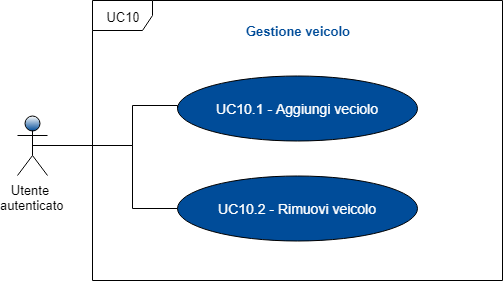
\includegraphics[width=10cm]{res/images/UC10Gestioneveicolo.png}
 	\centering
 	\caption{UC10 - Gestione Veicoli}
 \end{figure}
 \begin{itemize}
 	\item \textbf{Attori Primari}: utente autenticato;
 	\item \textbf{Descrizione}: l'utente visualizza i propri veicoli. Per ogni veicolo vengono visualizzate le seguenti informazioni:
 	\begin{itemize}
 		\item marca;
 		\item modello;
 		\item anno di immatricolazione;
 		\item rating.
 	\end{itemize}
 	\item \textbf{Precondizione}: l'utente accede al fragment\glosp per la gestione dei veicoli;
 	\item \textbf{Postcondizione}: l'utente visualizza le informazioni relative ai propri veicoli, con le eventuali operazioni disponibili su ognuno di essi.
 \end{itemize}
 \subsubsection{UC10.1 - Aggiunta veicolo}
 \begin{itemize}
 	\item \textbf{Attori Primari}: utente autenticato;
 	\item \textbf{Descrizione}: l'utente può aggiungere un mezzo di trasporto al proprio parco macchine;
 	\item \textbf{Scenario principale}: l'utente aggiunge un veicolo compilando gli appositi campi, ovvero:
 	\begin{itemize}
 		\item inserimento marca veicolo [UC10.1.1];
 		\item inserimento modello veicolo [UC10.1.2];
 		\item inserimento anno d'immatricolazione veicolo [UC10.1.3].
 	\end{itemize}
 	e successivamente salverà il nuovo veicolo [UC10.1.4];
 	\item \textbf{Precondizione}: l'utente ha inserito correttamente tutti i campi necessari;
 	\item \textbf{Postcondizione}: il nuovo veicolo viene aggiunto ai veicoli posseduti.
 \end{itemize}
\begin{figure}[H]
	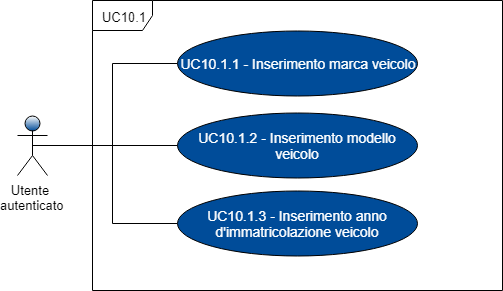
\includegraphics[width=10cm]{res/images/UC10-1Aggiungiveicolo.png}
	\centering
	\caption{UC10.1 - Aggiunta veicolo}
\end{figure}
\subsubsection{UC10.1.1 - Inserimento marca veicolo}
\begin{itemize}
	\item \textbf{Attori Primari}: utente autenticato;
	\item \textbf{Descrizione}: al fine di portare a termine il processo di inserimento di un nuovo veicolo l'utente deve inserirne la marca, campo ritenuto obbligatorio;
	\item \textbf{Scenario principale}: l'utente compila il campo relativo alla marca del veicolo;	
	\item \textbf{Precondizione}: l'applicazione ha reso disponibile il campo per l'inserimento della marca del veicolo;
	\item \textbf{Postcondizione}: l'utente ha compilato il campo con la marca.	
\end{itemize}

\subsubsection{UC10.1.2 - Inserimento modello veicolo}
\begin{itemize}
	\item \textbf{Attori Primari}: utente autenticato;
	\item \textbf{Descrizione}: al fine di portare a termine il processo di inserimento di un nuovo veicolo l'utente deve inserirne il modello, campo ritenuto obbligatorio;
	\item \textbf{Scenario principale}: l'utente compila il campo relativo alla marca del veicolo;	
	\item \textbf{Precondizione}: l'applicazione ha reso disponibile il campo per l'inserimento il modello del veicolo;
	\item \textbf{Postcondizione}: l'utente ha compilato il campo con il modello.	
\end{itemize}

\subsubsection{UC10.1.3 - Inserimento anno d'immatricolazione veicolo}
\begin{itemize}
	\item \textbf{Attori Primari}: utente autenticato;
	\item \textbf{Descrizione}: al fine di portare a termine il processo di inserimento di un nuovo veicolo l'utente deve inserirne l'anno di immatricolazione, campo ritenuto obbligatorio;
	\item \textbf{Scenario principale}: l'utente compila il campo relativo all'anno d'immatricolazione del veicolo;	
	\item \textbf{Precondizione}: l'applicazione ha reso disponibile il campo per l'inserimento dell'anno d'immatricolazione del veicolo;
	\item \textbf{Postcondizione}: l'utente ha compilato il campo con l'anno d'immatricolazione.	
\end{itemize}

\subsubsection{UC10.1.4 - Invio dati veicolo}
\begin{itemize}
	\item \textbf{Attori Primari}: utente autenticato;
	\item \textbf{Descrizione}: l'utente preme il pulsante per la conferma e l'invio dei dati del veicolo;
	\item \textbf{Scenario principale}: l'utente preme il pulsante di verifica ed invio dei dati;	
	\item \textbf{Precondizione}: i campi dati necessari per l'inserimento di un veicolo sono compilabili. È presente il pulsante per la conferma dei dati;
	\item \textbf{Postcondizione}: il nuovo veicolo viene inserito e l'utente potrà visualizzarlo nel proprio parco macchine.
\end{itemize}

\subsubsection{UC10.2 - Rimozione veicolo}
\begin{itemize}
	\item \textbf{Attori Primari}: utente autenticato;
	\item \textbf{Descrizione}: l'utente può rimuovere un mezzo di trasporto dal proprio parco macchine;
	\item \textbf{Scenario principale}: l'utente può selezionare un veicolo e attraverso l'apposito pulsante rimuoverlo dal proprio parco macchine.
	\item \textbf{Precondizione}: l'applicazione mostra all'utente i propri veicoli e ne permette la selezione.
	\item \textbf{Postcondizione}: il veicolo selezionato viene rimosso dal parco macchine
\end{itemize}
\begin{figure}[h]
	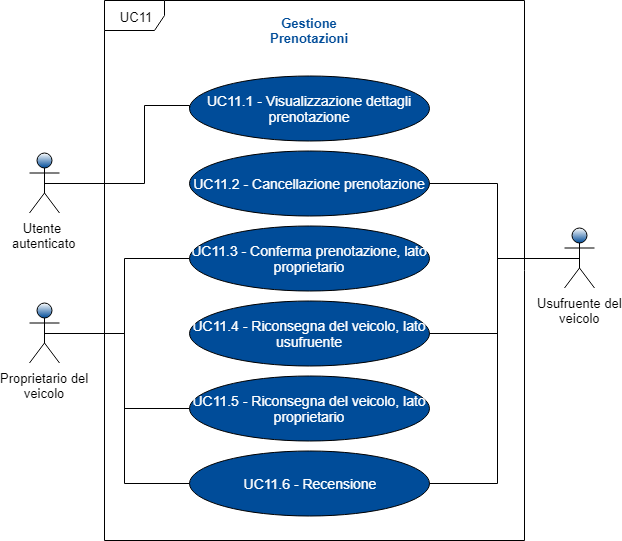
\includegraphics[width=12cm]{res/images/UC11Prenotazione.png}
	\centering
	\caption{UC11 - Gestione prenotazione}
\end{figure}
\subsubsection{UC11 - Gestione prenotazioni}
\begin{itemize}
	\item \textbf{Attori Primari}: utente autenticato;
	\item \textbf{Attori Secondari}:
	usufruente del veicolo, proprietario del veicolo;
	\item \textbf{Descrizione}: agli utenti autenticati è resa disponibile una maschera che presenta la lista di tutte le sue prenotazioni ancora attive, dalla quale l'utente può scegliere di effettuare operazioni di gestione su ognuna di esse;
	per ogni prenotazione presente nella lista saranno visualizzati dei dettagli riassuntivi, che sono:
	\begin{itemize}
		\item nome del proprietario del veicolo o dell'usufruente;
		\item data;
		\item fascia oraria;
		\item marca del veicolo prenotato;
		\item modello del veicolo prenotato;
		\item anno d'immatricolazione del veicolo prenotato.
	\end{itemize}
	\item \textbf{Scenario principale}: l'utente autenticato effettua operazioni di gestione di una prenotazione. Esse comprendono:
	\begin{itemize}
		\item visualizzazione dettagli prenotazione [UC11.1].
	\end{itemize}
	\item \textbf{Scenario alternativo}: Se l'utente autenticato è il proprietario del veicolo, inoltre potrà confermare:
	\begin{itemize}
		\item le prenotazioni ricevute [UC11.3];
		\item la riconsegna del veicolo [UC11.5];
		\item recensire l'usufruente [UC11.6].
	\end{itemize}
	Se l'utente autenticato è l'usufruente del veicolo, inoltre potrà:
	\begin{itemize}
		\item cancellare la prenotazione [UC11.2];
		\item richiedere la conferma della riconsegna del veicolo [UC11.4];
		\item recensire il proprietario [UC11.6].
	\end{itemize}
	\item \textbf{Precondizione}: il sistema carica correttamente la lista delle prenotazioni effettuate attualmente attive;
	\item \textbf{Postcondizione}: l'utente ha visualizzato le sue prenotazioni correnti ed è riuscito ad effettuare eventuali modifiche.
\end{itemize} 
 \subsubsection{UC11.1 - Visualizzazione dettagli prenotazione}
\begin{itemize}
	\item \textbf{Attori Primari}: utente autenticato;
	\item \textbf{Descrizione}: l'utente visualizza i dettagli della prenotazione scelta dalla maschera di presentazione delle prenotazioni, ciò gli permette di visualizzare:
	\begin{itemize}
		\item nome del proprietario del veicolo o dell'usufruente;
		\item la data;
		\item la fascia oraria;
		\item il veicolo prenotato.
	\end{itemize}
	Inoltre se presenti, verranno visualizzati anche:
	\begin{itemize}		
		\item il luogo d'incontro;
		\item l'orario d'incontro.
	\end{itemize}
	\item \textbf{Scenario principale}: l'utente visualizza i dettagli della prenotazione;	
	\item \textbf{Precondizione}: l'utente ha scelto una prenotazione;
	\item \textbf{Postcondizione}: l'utente ha visualizzato correttamente i dettagli della prenotazione.
\end{itemize}
\subsubsection{UC11.2 - Cancellazione prenotazione}
\begin{itemize}
	\item \textbf{Attori Primari}: usufruente del veicolo;
	\item \textbf{Descrizione}: l'utente usufruente cancella la prenotazione selezionata;
	\item \textbf{Scenario principale}: l'utente si trova all'interno della pagina di visualizzazione dei dettagli della prenotazione precedentemente selezionata. Attraverso l'apposito pulsante l'utente cancellerà la prenotazione effettuata;
	\item \textbf{Precondizione}: l'utente ha premuto il pulsante per la cancellazione delle prenotazione precedentemente selezionata;
	\item \textbf{Postcondizione}: l'utente ha annullato correttamente la prenotazione selezionata.
\end{itemize}
\subsubsection{UC11.3 - Conferma prenotazione, lato proprietario}
\begin{itemize}
	\item \textbf{Attori Primari}: proprietario del veicolo;
	\item \textbf{Descrizione}: il proprietario del veicolo conferma o annulla la richiesta di prenotazione ricevuta;
	\item \textbf{Scenario principale}: l'utente si trova all'interno della pagina di visualizzazione dei dettagli della richiesta di prenotazione appena ricevuta. Attraverso gli appositi campi l'utente potrà specificare:
	\begin{itemize}
		\item luogo d'incontro [UC11.3.1];
		\item orario d'incontro [UC11.3.2].
	\end{itemize} 
	successivamente conferma i dati e invia la risposta all'usufruente;
	\item \textbf{Precondizione}: l'utente visualizza correttamente la prenotazione che intende confermare o annullare;
	\item \textbf{Postcondizione}: l'utente ha confermato o annullato correttamente la richiesta di prenotazione ricevuta.
\end{itemize}
\begin{figure}[h]
	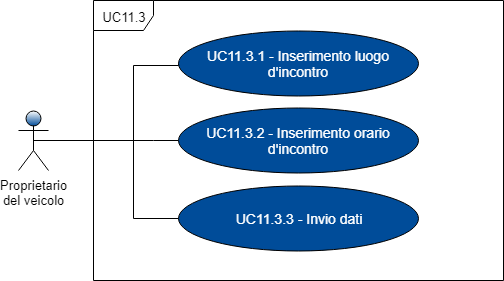
\includegraphics[width=10cm]{res/images/UC11-3Conferma.png}
	\centering
	\caption{UC11.3 - Conferma prenotazione, lato proprietario}
\end{figure}
\subsubsection{UC11.3.1 - Inserimento luogo d'incontro}
\begin{itemize}
	\item \textbf{Attori Primari}: proprietario del veicolo;
	\item \textbf{Descrizione}: al fine di portare a termine il processo di conferma della prenotazione, l'utente deve inserire il luogo d'incontro, campo ritenuto obbligatorio;
	\item \textbf{Scenario principale}: l'utente compila il campo relativo al luogo d'incontro;	
	\item \textbf{Precondizione}: l'applicazione ha reso disponibile il campo per l'inserimento del luogo d'incontro;
	\item \textbf{Postcondizione}: l'utente ha compilato il campo con il luogo d'incontro.	
\end{itemize}
\subsubsection{UC11.3.2 - Inserimento orario d'incontro}
\begin{itemize}
	\item \textbf{Attori Primari}: proprietario del veicolo;
	\item \textbf{Descrizione}: al fine di portare a termine il processo di conferma della prenotazione, l'utente deve inserire l'orario d'incontro, campo ritenuto obbligatorio;
	\item \textbf{Scenario principale}: l'utente compila il campo relativo all'orario d'incontro;	
	\item \textbf{Precondizione}: l'applicazione ha reso disponibile il campo per l'inserimento dell'orario d'incontro;
	\item \textbf{Postcondizione}: l'utente ha compilato il campo con l'orario d'incontro.	
\end{itemize}
\subsubsection{UC11.4 - Riconsegna del veicolo, lato usufruente}
\begin{itemize}
	\item \textbf{Attori Primari}: usufruente del veicolo;
	\item \textbf{Descrizione}: l'utente riconsegna il veicolo e chiude la prenotazione;
	\item \textbf{Scenario principale}: l'utente si trova all'interno della pagina di visualizzazione dei dettagli della prenotazione precedentemente selezionata. Dopo aver riconsegnato il veicolo e le chiavi, attraverso l'apposito pulsante l'utente chiederà la chiusura della prenotazione (la prenotazione verrà definitivamente chiusa quando anche il proprietario del veicolo confermerà la riconsegna delle chiavi e del mezzo [UC11.5]). Comparirà un pop-up che permetterà di lasciare una recensione all'altro utente [UC11.6];
	\item \textbf{Precondizione}: l'utente visualizza correttamente la prenotazione che intende concludere;
	\item \textbf{Postcondizione}: l'utente ha richiesto correttamente la chiusura della prenotazione selezionata.
\end{itemize}
\subsubsection{UC11.5 - Riconsegna del veicolo, lato proprietario}
\begin{itemize}
	\item \textbf{Attori Primari}: proprietario del veicolo;
	\item \textbf{Descrizione}: il proprietario del veicolo conferma la riconsegna del mezzo e delle chiavi;
	\item \textbf{Scenario principale}: l'utente si trova all'interno della pagina di visualizzazione dei dettagli della prenotazione precedentemente selezionata. Alla riconsegna del veicolo e delle chiavi, attraverso l'apposito pulsante l'utente confermerà la chiusura della prenotazione in modo definitivo. Comparirà un pop-up che permetterà di lasciare una recensione all'altro utente [UC11.6];
	\item \textbf{Precondizione}: l'utente visualizza correttamente la prenotazione che intende concludere;
	\item \textbf{Postcondizione}: l'utente ha concluso correttamente la prenotazione selezionata.
\end{itemize}

\subsubsection{UC11.6 - Recensione}
\begin{itemize}
	\item \textbf{Attori Primari}: utente autenticato;
	\item \textbf{Descrizione}: l'utente recensisce l'altro utente coinvolto nella prenotazione;
	\item \textbf{Scenario principale}: l'utente visualizza il pop-up per inserire la recensione che consiste in una valutazione da una a cinque stelle;
	\item \textbf{Precondizione}: l'utente visualizza correttamente il pop-up;
	\item \textbf{Postcondizione}: l'utente ha inserito correttamente la recensione.
\end{itemize}


\subsubsection{UC12 - Effettua una prenotazione}
\begin{figure}[h]
	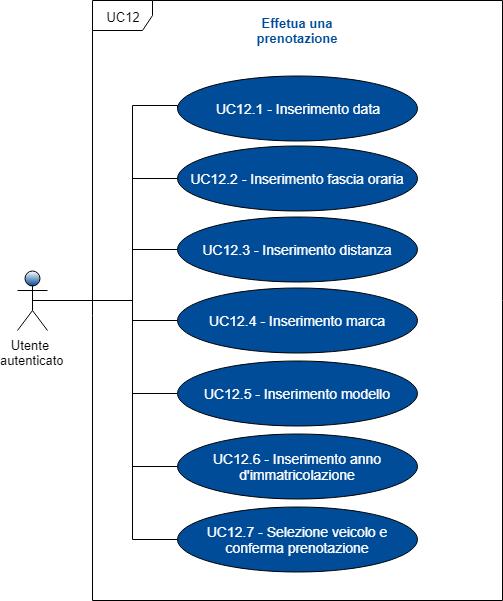
\includegraphics[width=10cm]{res/images/UC12Effettuaprenotazione.png}
	\centering
	\caption{UC12 - Effettua una prenotazione}
\end{figure}
\begin{itemize}
	\item \textbf{Attori Primari}: utente autenticato;
	\item \textbf{Descrizione}: l'utente può ricercare un veicolo sfruttando diversi parametri e prenotare quello più adatto alle sue esigenze.
	\item \textbf{Scenario principale}: l'utente per effettuare la prenotazione di un veicolo avrà a disposizione una maschera di ricerca che gli permetterà di filtrare i veicoli secondo questi parametri:
	\begin{itemize}
		\item data [UC12.1];
		\item ora di inizio [UC12.2];
		\item ora di fine [UC12.3];
		\item distanza: l'utente può inserire un raggio in chilometri per selezionare solo i veicoli presenti nell'area circoscritta [UC12.4]; 
		%\item marca [UC12.4];
		%\item modello [UC12.5];
		%\item anno d'immatricolazione [UC12.6].
	\end{itemize}
	L'utente avrà quindi a disposizione una lista di veicoli conformi alle sue preferenze di cui potrà visualizzare:
	\begin{itemize}		
		%\item nome del proprietario;
		\item marca;
		\item modello;
		\item anno d'immatricolazione;
		\item rating.
	\end{itemize}
	Successivamente l'utente selezionerà il veicolo più consono alle sue necessità e potrà inviare la richiesta di prenotazione [UC12.7].
	\item \textbf{Precondizione}: l'applicazione rende disponibile il filtro per la ricerca;
	\item \textbf{Post-condizione}: il veicolo risulta prenotato correttamente.
\end{itemize} 
\subsubsection{UC12.1 - Inserimento data}
\begin{itemize}
	\item \textbf{Attori Primari}: utente autenticato;
	\item \textbf{Descrizione}: al fine di rendere il filtro di ricerca più stringente, l'utente può inserire in un apposito campo la data in cui intende prenotare il veicolo;
	\item \textbf{Scenario principale}: l'utente compila il campo relativo alla data;	
	\item \textbf{Precondizione}: l'applicazione ha reso disponibile il campo per l'inserimento della data;
	\item \textbf{Postcondizione}: l'utente ha compilato il campo con la data in cui intende prenotare un veicolo.	
\end{itemize}
\subsubsection{UC12.2 - Inserimento fascia oraria}
\begin{itemize}
	\item \textbf{Attori Primari}: utente autenticato;
	\item \textbf{Descrizione}: al fine di rendere il filtro di ricerca più stringente, l'utente può inserire in un apposito campo la fascia oraria in cui s'intende prenotare il veicolo;
	\item \textbf{Scenario principale}: l'utente compila il campo relativo alla fascia oraria;	
	\item \textbf{Precondizione}: l'applicazione ha reso disponibile il campo per l'inserimento della fascia oraria;
	\item \textbf{Postcondizione}: l'utente ha compilato il campo con la fascia oraria in cui intende prenotare un veicolo.	
\end{itemize}
\subsubsection{UC12.3 - Inserimento distanza}
\begin{itemize}
	\item \textbf{Attori Primari}: utente autenticato;
	\item \textbf{Descrizione}: al fine di rendere il filtro di ricerca più stringente, l'utente può inserire in un apposito campo il raggio in chilometri secondo cui circoscrivere i veicoli;
	\item \textbf{Scenario principale}: l'utente compila il campo relativo alla distanza;	
	\item \textbf{Precondizione}: l'applicazione ha reso disponibile il campo per l'inserimento della distanza;
	\item \textbf{Postcondizione}: l'utente ha compilato il campo con la distanza.	
\end{itemize}
\subsubsection{UC12.4 - Inserimento marca}
\begin{itemize}
	\item \textbf{Attori Primari}: utente autenticato;
	\item \textbf{Descrizione}: al fine di rendere il filtro di ricerca più stringente, l'utente può inserire in un apposito campo la marca del veicolo che intende prenotare;
	\item \textbf{Scenario principale}: l'utente compila il campo relativo alla marca;	
	\item \textbf{Precondizione}: l'applicazione ha reso disponibile il campo per l'inserimento della marca;
	\item \textbf{Postcondizione}: l'utente ha compilato il campo con una marca di veicoli.	
\end{itemize}
\subsubsection{UC12.5 - Inserimento modello}
\begin{itemize}
	\item \textbf{Attori Primari}: utente autenticato;
	\item \textbf{Descrizione}: al fine di rendere il filtro di ricerca più stringente, l'utente può inserire in un apposito campo il modello del veicolo che intende prenotare;
	\item \textbf{Scenario principale}: l'utente compila il campo relativo al modello;	
	\item \textbf{Precondizione}: l'applicazione ha reso disponibile il campo per l'inserimento del modello;
	\item \textbf{Postcondizione}: l'utente ha compilato il campo con il modello di veicolo cercato.	
\end{itemize}
\subsubsection{UC12.6 - Inserimento anno d'immatricolazione}
\begin{itemize}
	\item \textbf{Attori Primari}: utente autenticato;
	\item \textbf{Descrizione}: al fine di rendere il filtro di ricerca più stringente, l'utente può inserire in un apposito campo l'anno d'immatricolazione per specificare che i veicoli cercati devono essere stati immatricolati in quell'anno o in un periodo più recente;
	\item \textbf{Scenario principale}: l'utente compila il campo relativo all'anno d'immatricolazione;	
	\item \textbf{Precondizione}: l'applicazione ha reso disponibile il campo per l'inserimento dell'anno d'immatricolazione;
	\item \textbf{Postcondizione}: l'utente ha compilato il campo con l'anno d'immatricolazione.	
\end{itemize}
\subsubsection{UC12.7 - Selezione veicolo}
\begin{itemize}
	\item \textbf{Attori Primari}: utente autenticato;
	\item \textbf{Descrizione}: una volta filtrati i veicoli, l'utente potrà scegliere quello più di suo gradimento, selezionarlo e prenotarlo tramite l'apposito pulsante;
	\item \textbf{Scenario principale}: 
	l'utente seleziona un veicolo e lo prenota con l'apposito pulsante;
	\item \textbf{Precondizione}: l'applicazione ha reso disponibile all'utente almeno un veicolo selezionabile;
	\item \textbf{Postcondizione}: l'utente ha prenotato correttamente il veicolo.
\end{itemize}


\subsubsection{UC14 - Storico prenotazioni}
 \begin{figure}[h]
	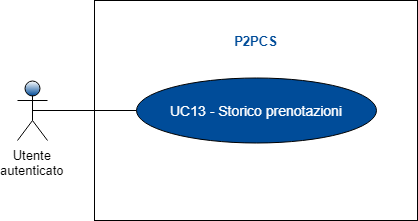
\includegraphics[width=8cm]{res/images/Schemagenerale4.png}
	\centering
	\caption{UC14 - Storico prenotazioni}
\end{figure}
\begin{itemize}
	\item \textbf{Attori Primari}: utente autenticato;
	\item \textbf{Descrizione}: agli utenti autenticati è resa disponibile una maschera che presenta la lista di tutte le sue prenotazioni concluse dalla quale si possono ricavare le seguenti informazioni:
	\begin{itemize}
		\item marca;
		\item modello;
		\item data;
		\item fascia oraria;
		\item stato della prenotazione;
		\item immagine del veicolo.
	\end{itemize} 
	\item \textbf{Scenario principale}: l'utente visualizza la lista contenente tutte le sue prenotazioni concluse;
	\item \textbf{Precondizione}: l'utente autenticato ha selezionato la voce \textit{Storico prenotazioni} dal menu dell'applicazione;
	\item \textbf{Post-condizione}: l'utente autenticato ha visualizzato lo storico delle sue prenotazioni concluse. 
\end{itemize} 

\begin{figure}[h]
	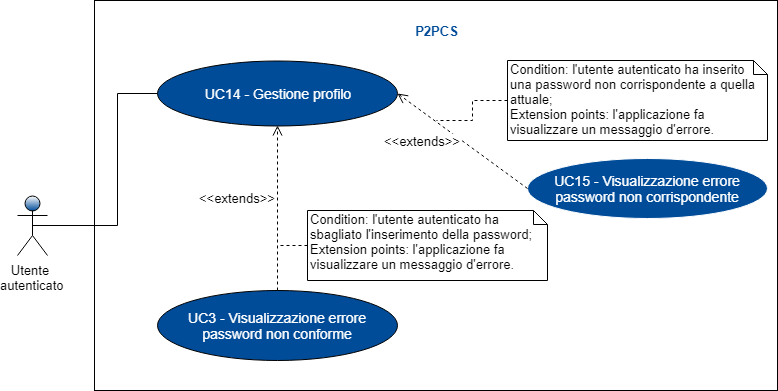
\includegraphics[width=15cm]{res/images/Schemagenerale5.png}
	\centering
	\caption{Schema generale: gestione profilo ed errori annessi}
\end{figure}
\subsubsection{UC14 - Gestione Profilo}
\begin{itemize}
	\item \textbf{Attori Primari}: utente autenticato;
	\item \textbf{Descrizione}: agli utenti autenticati è resa disponibile una maschera che presenta il proprio profilo, dalla quale l'utente può scegliere di modificarlo o eliminarlo;
	\item \textbf{Scenario principale}: l'utente visualizza il profilo e ha la possibilità di: 
	\begin{itemize}
		\item Modifica dati account [UC14.1];
		\item Eliminazione account [UC14.2].
	\end{itemize}
	\item \textbf{Precondizione}: l'utente è in possesso di un account all'interno del sistema. Deve quindi essersi registrato e non aver eliminato l'account;
	\item \textbf{Postcondizione}: l'utente ha effettuato l'operazione di modifica dati oppure l'eliminazione dell'account e il processo è stato confermato dal sistema.
	\item \textbf{Estensioni}:
	\begin{itemize}
		\item Visualizzazione errore password non conforme [UC3];
		\item Visualizzazione errore password non corrispondente [UC15].
	\end{itemize}
\end{itemize}
\begin{figure}[h]
	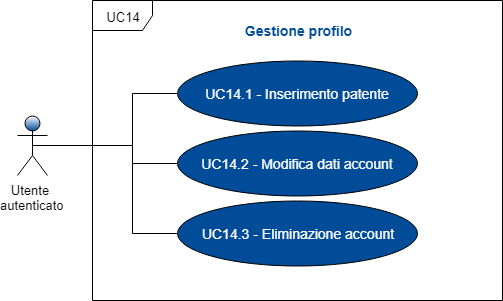
\includegraphics[width=10cm]{res/images/UC14Profilo.png}
	\centering
	\caption{UC14 - Gestione Profilo}
\end{figure} 
\subsubsection{UC14.1 - Modifica dati account}
\begin{itemize}
	\item \textbf{Attori Primari}: utente autenticato;
	\item \textbf{Descrizione}: l'utente ha la possibilità di modificare i propri dati;
	\item \textbf{Scenario principale}: l'utente può modificare:
	\begin{itemize}
		\item Nome [UC14.1.1];
		\item Cognome [UC14.1.2];
		\item Numero telefonico [UC14.1.3];
		\item E-mail [UC14.1.4];
		\item Data di nascita [UC14.1.5];
		\item Residenza [UC14.1.6];
		\item Password [UC14.1.7].
	\end{itemize}
	e confermare la modifica dei dati [UC14.1.8];
	\item \textbf{Scenari alternativi}: l'utente interrompe la modifica dei dati senza confermare il salvataggio di essi. Il sistema non salverà le modifiche parziali apportate dall'utente me lo riporterà alla schermata di visualizzazione dell'account;	 
	\item \textbf{Precondizione}: l'utente è in possesso di un account all'interno del sistema. Deve quindi essersi registrato e non aver eliminato l'account;
	\item \textbf{Postcondizione}: il sistema ha memorizzato le modifiche apportate ai dati da parte dell’utente;
	\item \textbf{Inclusioni}:
	\begin{itemize}
		\item Inserimento vecchia password [U14.1.7.1];
		\item Inserimento nuova password [UC14.1.7.2].
	\end{itemize}
\end{itemize}
\begin{figure}[h]
	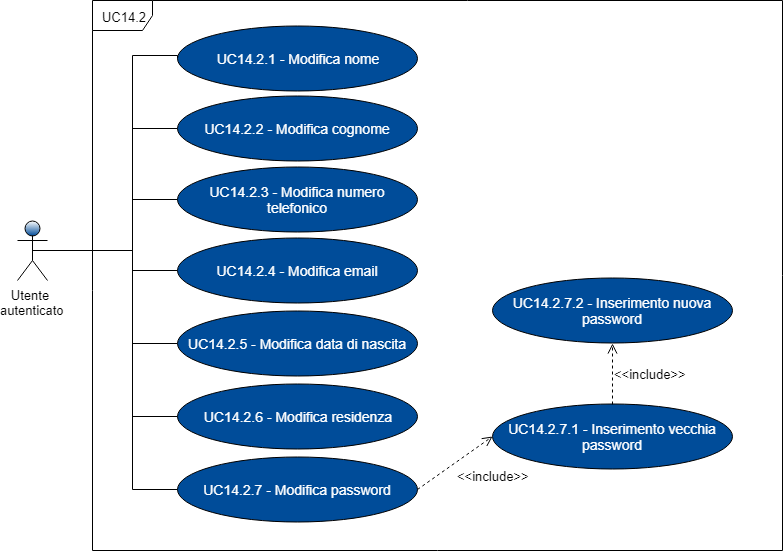
\includegraphics[width=14cm]{res/images/UC14-1Modifica.png}
	\centering
	\caption{UC14.1 - Modifica dati account}
\end{figure}
\newpage 
\subsubsection{UC14.1.1 - Modifica nome}
\begin{itemize}
	\item \textbf{Attori Primari}: utente autenticato;
	\item \textbf{Descrizione}: l'utente ha la possibilità di modificare il nome inserito in precedenza;
	\item \textbf{Precondizione}: il sistema fornisce una schermata nella quale è possibile inserire il nuovo nome;
	\item \textbf{Postcondizione}: l'utente ha inserito il nuovo nome.
\end{itemize}

\subsubsection{UC14.1.2 - Modifica cognome}
\begin{itemize}
	\item \textbf{Attori Primari}: utente autenticato;
	\item \textbf{Descrizione}: l'utente ha la possibilità di modificare il cognome inserito in precedenza;
	\item \textbf{Precondizione}: il sistema fornisce una schermata nella quale è possibile inserire il nuovo cognome;
	\item \textbf{Postcondizione}: l'utente ha inserito il nuovo cognome.
\end{itemize}

\subsubsection{UC14.1.3 - Modifica numero telefonico}
\begin{itemize}
	\item \textbf{Attori Primari}: utente autenticato;
	\item \textbf{Descrizione}: l'utente ha la possibilità di modificare il numero telefonico inserito in precedenza;
	\item \textbf{Precondizione}: il sistema fornisce una schermata nella quale è possibile inserire il nuovo numero telefonico;
	\item \textbf{Postcondizione}: l'utente ha inserito il nuovo numero telefonico.
\end{itemize}

\subsubsection{UC14.1.4 - Modifica email}
\begin{itemize}
	\item \textbf{Attori Primari}: utente autenticato;
	\item \textbf{Descrizione}: l'utente ha la possibilità di modificare l'email inserita in precedenza;
	\item \textbf{Precondizione}: il sistema fornisce una schermata nella quale è possibile inserire la nuova email;
	\item \textbf{Postcondizione}: l'utente ha inserito la nuova email.
\end{itemize}

\subsubsection{UC14.1.5 - Modifica data di nascita}
\begin{itemize}
	\item \textbf{Attori Primari}: utente autenticato;
	\item \textbf{Descrizione}: l'utente ha la possibilità di modificare la data di nascita inserita in precedenza;
	\item \textbf{Precondizione}: il sistema fornisce una schermata nella quale è possibile inserire la nuova data di nascita;
	\item \textbf{Postcondizione}: l'utente ha inserito la nuova data di nascita.
\end{itemize}

\subsubsection{UC14.1.6 - Modifica residenza}
\begin{itemize}
	\item \textbf{Attori Primari}: utente autenticato;
	\item \textbf{Descrizione}: l'utente ha la possibilità di modificare la residenza inserita in precedenza;
	\item \textbf{Precondizione}: il sistema fornisce una schermata nella quale è possibile inserire la nuova residenza;
	\item \textbf{Postcondizione}: l'utente ha inserito la nuova residenza.
\end{itemize}

\subsubsection{UC14.1.7 - Modifica password}
\begin{itemize}
	\item \textbf{Attori Primari}: utente autenticato;
	\item \textbf{Descrizione}: l'utente ha la possibilità di modificare la password inserita in precedenza inserendo prima la vecchia password e poi quella nuova;
	\item \textbf{Scenario principale}: il sistema fornisce per prima cosa all'utente la possibilità di:
		\begin{itemize}
			\item Inserimento vecchia password [UC14.1.7.1].
		\end{itemize}
	e poi di:
		\begin{itemize}
			\item Inserimento nuova password [UC14.1.7.2].
		\end{itemize}
	\item \textbf{Precondizione}: il sistema fornisce una schermata nella quale è possibile inserire la nuova password;
	\item \textbf{Postcondizione}: l'utente ha inserito la nuova password.
\end{itemize}

\subsubsection{UC14.1.7.1 - Inserimento vecchia password}
\begin{itemize}
	\item \textbf{Attori Primari}: utente autenticato;
	\item \textbf{Descrizione}: l'utente deve inserire la password attuale per poterla aggiornare;
	\item \textbf{Precondizione}: il sistema fornisce una schermata nella quale è possibile inserire la vecchia password;
	\item \textbf{Postcondizione}: l'utente ha inserito la vecchia password.
\end{itemize}

\subsubsection{UC14.1.7.2 - Inserimento nuova password}
\begin{itemize}
	\item \textbf{Attori Primari}: utente autenticato;
	\item \textbf{Descrizione}: l'utente deve inserire la nuova password, diversa da quella attuale, per effettuare l'aggiornamento;
	\item \textbf{Precondizione}: il sistema fornisce una schermata nella quale è possibile inserire la nuova password;
	\item \textbf{Postcondizione}: l'utente ha inserito la nuova password.
\end{itemize}

\subsubsection{UC14.1.8 - Conferma modifica dati}
\begin{itemize}
	\item \textbf{Attori Primari}: utente autenticato;
	\item \textbf{Descrizione}: l'utente deve 
	confermare la modifica apportata;
	\item \textbf{Precondizione}: l'utente ha inserito tutti i dati richiesti e desiderati. Si trova dunque davanti ad una schermata con la possibilità di confermare la modifica effettuata;
	\item \textbf{Postcondizione}: l'utente ha confermato di voler rendere effettivo il cambiamento del proprio account.
\end{itemize}

\subsubsection{UC14.2 - Eliminazione account}
\begin{itemize}
	\item \textbf{Attori Primari}: utente autenticato;
	\item \textbf{Descrizione}: all'utente viene fornita la possibilità di eliminare il proprio account e di conseguenza i propri dati all'interno del sistema.
	\item \textbf{Precondizione}: l'utente è in possesso di un account all'interno del sistema. Deve quindi aver effettuato la registrazione e non avere mai effettuato la procedura di eliminazione account.
	\item \textbf{Postcondizione}: l'utente ha cancellato il proprio account e viene riportato alla schermata iniziale dell'applicazione [UC1]. Il sistema non terrà taccia del profilo eliminato.
\end{itemize}

\subsubsection{UC15 - Visualizzazione errore password non corrispondente}
\begin{itemize}
	\item \textbf{Attori Primari}: utente autenticato;
	\item \textbf{Descrizione}: l'utente visualizza un messaggio d'errore in quanto la password digitata in [UC14.1.7.1] non corrisponde alla vecchia password;
	\item \textbf{Scenario principale}: l'utente autenticato cerca di cambiare la password del proprio account;
	\item \textbf{Precondizione}: l'utente autenticato ha inserito una password non corrispondente a quella attuale;
	\item \textbf{Postcondizione}: l'applicazione fa visualizzare un messaggio d'errore.
\end{itemize}




\begin{figure}[h]
	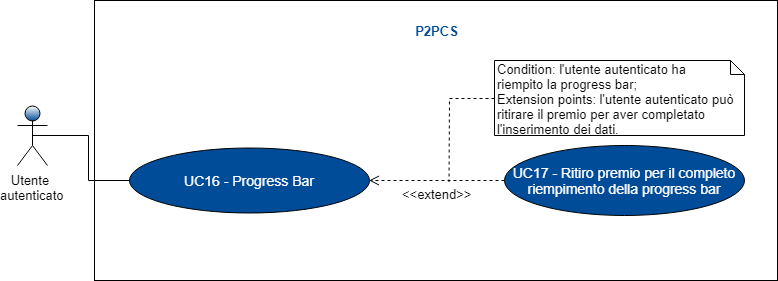
\includegraphics[width=13cm]{res/images/Schemagenerale7.png}
	\centering
	\caption{Schema generale: progress bar}
\end{figure}
\subsubsection{UC16 - Progress Bar}
\begin{itemize}
	\item \textbf{Attori Primari}: utente autenticato;
	\item \textbf{Descrizione}: l'utente che non ha ancora inserito tutti i suoi dati nel profilo visualizzerà una barra di avanzamento che si riempirà progressivamente in base ai dati inseriti;
	\item \textbf{Scenario principale}: l'utente apre la sezione \textit{Gestione Profilo} [UC14] e non ha ancora inserito tutti i dati possibili;
	\item \textbf{Estensioni}:
	\begin{itemize}
		\item ritiro del premio per il completo riempimento della progress bar [UC17].
	\end{itemize}
	\item \textbf{Precondizione}: l'utente autenticato non ha inserito tutti i dati possibili;
	\item \textbf{Postcondizione}: l'utente autenticato visualizza la progress bar.	
\end{itemize}

\subsubsection{UC17 - Ritiro premio per il completo riempimento della progress bar}
\begin{itemize}
	\item \textbf{Attori Primari}: utente autenticato;
	\item \textbf{Descrizione}: l'utente autenticato ha completato l'inserimento dei dati e può ritirare il relativo premio;	
	\item \textbf{Scenario principale}: l'utente autenticato ha riempito con successo la progress bar e gli compare la schermata per il ritiro della ricompensa;
	\item \textbf{Precondizione}: l'utente autenticato ha riempito la progress bar;
	\item \textbf{Postcondizione}: l'utente autenticato può ritirare il premio per aver completato l'inserimento dei dati.
\end{itemize}

\begin{figure}[h]
	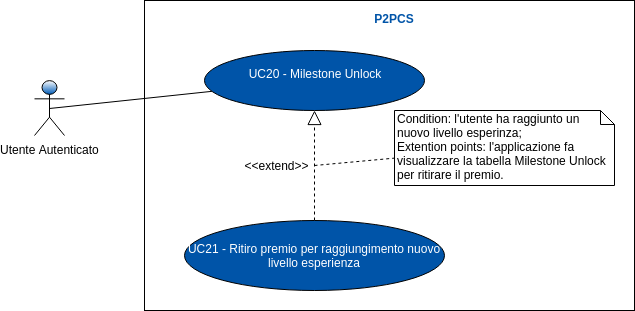
\includegraphics[width=10cm]{res/images/uc20-21.png}
	\centering
	\caption{Schema generale: milestone unlock}
\end{figure}
\subsubsection{UC20 - Milestone Unlock}
\begin{itemize}
	\item \textbf{Attori Primari}: utente autenticato;
	\item \textbf{Descrizione}: l'utente generico può visualizzare la tabella Milestone Unlock\glo, che illustra per ogni livello esperienza il corrispettivo premio che si può ottenere;	
	\item \textbf{Scenario principale}: l'utente ha premuto il pulsante per la visualizzazione della tabella Milestone Unlock, e la sta visualizzando.
	I premi presenti nella tabella possono essere del seguente tipo:
	\begin{itemize}
		\item aumento del valore del prossimo buono sconto che si andrà a ricevere (x\% in più);
		\item sconto dell'x\% sul prossimo acquisto nel negozio dell'applicazione;
		\item beni virtuali.
	\end{itemize}
	I premi partono dal quinto livello esperienza.
	Ogni 10 livelli esperienza, il valore del premio è aumentato del 10\%;
	\item \textbf{Precondizione}: l'utente autenticato ha premuto il pulsante della Milestone Unlock, dal menu dell'applicazione;
	\item \textbf{Postcondizione}: l'utente autenticato sta visualizzando la tabella Milestone Unlock;
	\item \textbf{Estensioni}:
		\begin{itemize}
			\item l'utente autenticato ha raggiunto un nuovo livello esperienza e ritira il premio corrispondente al livello raggiunto tramite la tabella Milestone Unlock [UC21].
		\end{itemize}
\end{itemize}
\subsubsection{UC21 - Ritiro premio per raggiungimento nuovo livello esperienza}
\begin{itemize}
	\item \textbf{Attori Primari}: utente autenticato;
	\item \textbf{Descrizione}: l'utente autenticato ha raggiunto un nuovo livello esperienza presente nella tabella Milestone Unlock\glosp e può ritirare il relativo premio;	
	\item \textbf{Scenario principale}: l'utente autenticato ha raggiunto un nuovo livello esperienza e gli si presenta la tabella di Milestone Unlock, dalla quale può ritirare il corrispondente premio. Il premio appena sbloccato sarà illuminato da un'aura gialla;
	\item \textbf{Precondizione}: l'utente autenticato ha raggiunto un nuovo livello esperienza, superiore al 5;
	\item \textbf{Postcondizione}: l'utente autenticato può ritirare il premio corrispondete al livello raggiunto, tramite la tabella Milestone Unlock.
\end{itemize}

\begin{figure}[h]
	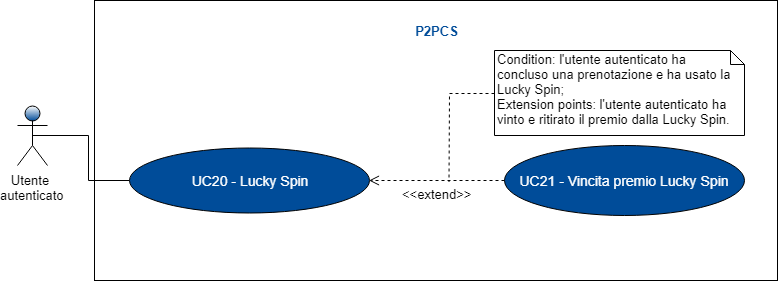
\includegraphics[width=9cm]{res/images/UC20Luckyspin.png}
	\centering
	\caption{UC22 - Lucky Spin}
\end{figure}
\subsubsection{UC22 - Lucky Spin}
\begin{itemize}
	\item \textbf{Attori Primari}: utente autenticato;
	\item \textbf{Descrizione}:	l'utente può visualizzare la lista dei premi ottenibili tramite la Lucky Spin\glo. Se è trascorso l'ammontare di tempo imposto dallo sviluppatore, può usare la Lucky Spin per ottenere un premio. Se non fosse interessato in quel momento a girare la ruota, può farlo in un secondo momento cliccando sul pulsante all'interno dell'area \textit{Gioca};
	\item \textbf{Scenario principale}: l'utente preme il pulsante \textit{Lucky Spin}. Nel caso sia trascorso il tempo imposto, può usare la Lucky Spin per ottenere un premio. I premi ottenibili sono del seguente tipo:
	\begin{itemize}
		\item accessori per personalizzare l'auto nel Minigioco;
		\item punti esperienza bonus;
		\item vincita di un viaggio gratuito con \textit{GaiaGo};
		\item buono sconto su un sito di e-commerce.	
	\end{itemize}
	\item \textbf{Precondizione}: l'utente ha premuto il pulsante della Lucky Spin;
	\item \textbf{Postcondizione}: l'utente sta visualizzando la lista dei premi ottenibili tramite la Lucky Spin.
\end{itemize}
\subsubsection{UC23 - Vincita premio Lucky Spin}
\begin{figure}[h]
	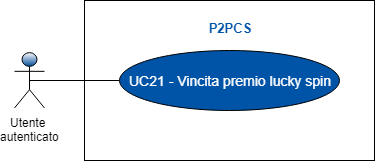
\includegraphics[width=9cm]{res/images/uc21.png}
	\centering
	\caption{UC23 - Vincita premio Lucky Spin}
\end{figure}
\begin{itemize}
	\item \textbf{Attori Primari}: utente autenticato;
	\item \textbf{Descrizione}: l'utente ha aspettato il tempo necessario e può usare la Lucky Spin\glosp per ottenere un premio;	
	\item \textbf{Scenario principale}: l'utente visualizza la schermata della Lucky Spin, nella quale può premere il pulsante \textit{Gira} per usare i suoi tentativi disponibili. Il premio gli verrà mostrato tramite un pop-up che metterà in risalto il premio vinto;
	\item \textbf{Precondizione}: l'utente autenticato ha aspettato il tempo necessario e ha usato la Lucky Spin;
	\item \textbf{Postcondizione}: l'utente autenticato ha vinto e ritirato il premio dalla Lucky Spin.
\end{itemize}


\subsubsection{UC24 - Leaderboard}
\begin{itemize}
	\item \textbf{Attori Primari}: utente autenticato;
	\item \textbf{Descrizione}: l'utente visualizza la classifica dei migliori utenti all'interno della sua area personale;
	\item \textbf{Scenario principale}: l'utente apre la sezione gestione profilo [UC14] e consulta la classifica utenti;
	\item \textbf{Precondizione}: l'applicazione rende disponibile la visualizzazione della leaderboard;
	\item \textbf{Postcondizione}: l'utente autenticato ha visualizzato la leaderboard;
\end{itemize}


\begin{figure}[h]
	%\includegraphics[width=8cm]{res/images/Codiceamico.png}
	\centering
	\caption{Schema generale: codice invito amici}
\end{figure}
\subsubsection{UC - Codice invito amici}
\begin{itemize}
	\item \textbf{Attori Primari}: utente autenticato;
	\item \textbf{Descrizione}: agli utenti autenticati è reso disponibile un codice personale (composto da lettere e numeri) che può essere inviato ad un amico, non ancora registrato, per invitarlo ad usufruire dell'applicazione semplicemente inserendo questo "codice amico" in fase di registrazione nell'apposito spazio facendo guadagnare così punti bonus al proprietario del codice;
	\item \textbf{Scenario principale}: l'utente visualizza, nella voce \textit{Gestione Profilo}, il codice personale da inviare ad amici;
	\item \textbf{Precondizione}: l'utente autenticato ha selezionato la voce \textit{Gestione Profilo} dal menu dell'applicazione;
	\item \textbf{Post-condizione}: l'utente autenticato ha visualizzato il suo codice personale. 
\end{itemize} 

